\documentclass[11pt,addpoints]{exam}
\usepackage{fullpage}
\usepackage{amsfonts, amsmath, amssymb, amsthm}
\usepackage{mathtools}
\usepackage{enumerate}
\usepackage{listings}
\usepackage[boxed]{algorithm}
\usepackage[noend]{algpseudocode}
\usepackage{hyperref}
\usepackage{tikz}
\usepackage[inline,shortlabels]{enumitem}
\usepackage{subcaption}

% in order to compile this file you need to get 'header.tex' from
% Canvas and change the line below to the appropriate file path
%%% theorems

\theoremstyle{plain}            % following are "theorem" style
\newtheorem{theorem}{Theorem}[section]
\newtheorem{lemma}[theorem]{Lemma}
\newtheorem{corollary}[theorem]{Corollary}
\newtheorem{proposition}[theorem]{Proposition}
\newtheorem{claim}[theorem]{Claim}
\newtheorem{fact}[theorem]{Fact}
\newtheorem{openproblem}[theorem]{Open Problem}

\theoremstyle{definition}       % following are def style
\newtheorem{definition}[theorem]{Definition}
\newtheorem{conjecture}[theorem]{Conjecture}
\newtheorem{example}[theorem]{Example}
\newtheorem{protocol}[theorem]{Protocol}
\newtheorem{exercise}[theorem]{Exercise}

\theoremstyle{remark}           % following are remark style
\newtheorem{remark}[theorem]{Remark}
\newtheorem{note}[theorem]{Note}
\newtheorem*{aside}{Aside}
\newtheorem*{gn}{Grading Note} % grading note

%%% special sets
\newcommand{\bit}{\ensuremath{\{0,1\}}}
\newcommand{\bitt}{\ensuremath{\{-1,1\}}}

% font for general-purpose algorithms
\newcommand{\algo}[1]{\ensuremath{\mathsf{#1}}}
% font for general-purpose computational problems
\newcommand{\problem}[1]{\ensuremath{\mathsf{#1}}}
% font for complexity classes
%\newcommand{\class}[1]{\ensuremath{\mathsf{#1}}}

\global\long\def\path{\mathrm{path}}
% asymptotics
%\DeclareMathOperator{\poly}{poly}
%\DeclareMathOperator{\polylog}{polylog}
\DeclareMathOperator{\negl}{negl}
\DeclareMathOperator{\Otil}{\tilde{O}}
\DeclareMathOperator{\Ostar}{O^*}

%%% "LEFT-RIGHT" PAIRS OF SYMBOLS

% inner product
\DeclarePairedDelimiter\inner{\langle}{\rangle}
% absolute value
\DeclarePairedDelimiter\abs{\lvert}{\rvert}
% a set
\DeclarePairedDelimiter\set{\{}{\}}
% parens
\DeclarePairedDelimiter\parens{(}{)}
% tuple, alias for parens
\DeclarePairedDelimiter\tuple{(}{)}
% square brackets
\DeclarePairedDelimiter\bracks{[}{]}
% rounding off
\DeclarePairedDelimiter\round{\lfloor}{\rceil}
% floor function
\DeclarePairedDelimiter\floor{\lfloor}{\rfloor}
% ceiling function
\DeclarePairedDelimiter\ceil{\lceil}{\rceil}
% length of some vector, element
\DeclarePairedDelimiter\length{\lVert}{\rVert}
% norm
\DeclarePairedDelimiter\norm{\lVert}{\rVert}
% length (as a string)
\DeclarePairedDelimiter\len{\lvert}{\rvert}
% bra-kets
\DeclarePairedDelimiter\bra{\langle}{\rvert}
\DeclarePairedDelimiter\ket{\lvert}{\rangle}
\newcommand{\braket}[2]{\ensuremath{\langle #1 \vert #2 \rangle}}
\newcommand{\ketbra}[2]{\ensuremath{\lvert #1 \rangle \langle #2 \rvert}}

%%% MATH OPERATORS
\DeclareMathOperator{\Var}{Var}
\DeclareMathOperator{\tr}{Tr}
\DeclareMathOperator{\supp}{supp}
\DeclareMathOperator{\var}{var}
\DeclareMathOperator{\vol}{vol}
\DeclareMathOperator{\sign}{sign}

%%% BLACKBOARD SYMBOLS

\newcommand{\C}{\ensuremath{\mathbb{C}}}
\newcommand{\D}{\ensuremath{\mathbb{D}}}
\newcommand{\F}{\ensuremath{\mathbb{F}}}
\newcommand{\G}{\ensuremath{\mathbb{G}}}
\newcommand{\J}{\ensuremath{\mathbb{J}}}
\newcommand{\N}{\ensuremath{\mathbb{N}}}
\newcommand{\Q}{\ensuremath{\mathbb{Q}}}
\newcommand{\R}{\ensuremath{\mathbb{R}}}
\newcommand{\T}{\ensuremath{\mathbb{T}}}
\newcommand{\Z}{\ensuremath{\mathbb{Z}}}
\newcommand{\QR}{\ensuremath{\mathbb{QR}}}

% sets in calligraphic type

\newcommand{\calD}{\ensuremath{\mathcal{D}}}
\newcommand{\calF}{\ensuremath{\mathcal{F}}}
\newcommand{\calG}{\ensuremath{\mathcal{G}}}
\newcommand{\calH}{\ensuremath{\mathcal{H}}}
\newcommand{\calI}{\ensuremath{\mathcal{I}}}
\newcommand{\calL}{\ensuremath{\mathcal{L}}}
\newcommand{\calN}{\ensuremath{\mathcal{N}}}
\newcommand{\calP}{\ensuremath{\mathcal{P}}}
\newcommand{\calS}{\ensuremath{\mathcal{S}}}
\newcommand{\calX}{\ensuremath{\mathcal{X}}}
\newcommand{\calY}{\ensuremath{\mathcal{Y}}}

% matrices and vectors

\newcommand{\matA}{\ensuremath{\mathbf{A}}}
\newcommand{\matB}{\ensuremath{\mathbf{B}}}
\newcommand{\matC}{\ensuremath{\mathbf{C}}}
\newcommand{\matD}{\ensuremath{\mathbf{D}}}
\newcommand{\matE}{\ensuremath{\mathbf{E}}}
\newcommand{\matF}{\ensuremath{\mathbf{F}}}
\newcommand{\matG}{\ensuremath{\mathbf{G}}}
\newcommand{\matH}{\ensuremath{\mathbf{H}}}
\newcommand{\matI}{\ensuremath{\mathbf{I}}}
\newcommand{\matJ}{\ensuremath{\mathbf{J}}}
\newcommand{\matK}{\ensuremath{\mathbf{K}}}
\newcommand{\matL}{\ensuremath{\mathbf{L}}}
\newcommand{\matM}{\ensuremath{\mathbf{M}}}
\newcommand{\matN}{\ensuremath{\mathbf{N}}}
\newcommand{\matO}{\ensuremath{\mathbf{O}}}
\newcommand{\matP}{\ensuremath{\mathbf{P}}}
\newcommand{\matQ}{\ensuremath{\mathbf{Q}}}
\newcommand{\matR}{\ensuremath{\mathbf{R}}}
\newcommand{\matS}{\ensuremath{\mathbf{S}}}
\newcommand{\matT}{\ensuremath{\mathbf{T}}}
\newcommand{\matU}{\ensuremath{\mathbf{U}}}
\newcommand{\matV}{\ensuremath{\mathbf{V}}}
\newcommand{\matW}{\ensuremath{\mathbf{W}}}
\newcommand{\matX}{\ensuremath{\mathbf{X}}}
\newcommand{\matY}{\ensuremath{\mathbf{Y}}}
\newcommand{\matZ}{\ensuremath{\mathbf{Z}}}
\newcommand{\matzero}{\ensuremath{\mathbf{0}}}

\newcommand{\veca}{\ensuremath{\mathbf{a}}}
\newcommand{\vecb}{\ensuremath{\mathbf{b}}}
\newcommand{\vecc}{\ensuremath{\mathbf{c}}}
\newcommand{\vecd}{\ensuremath{\mathbf{d}}}
\newcommand{\vece}{\ensuremath{\mathbf{e}}}
\newcommand{\vecf}{\ensuremath{\mathbf{f}}}
\newcommand{\vecg}{\ensuremath{\mathbf{g}}}
\newcommand{\vech}{\ensuremath{\mathbf{h}}}
\newcommand{\veck}{\ensuremath{\mathbf{k}}}
\newcommand{\vecm}{\ensuremath{\mathbf{m}}}
\newcommand{\vecp}{\ensuremath{\mathbf{p}}}
\newcommand{\vecq}{\ensuremath{\mathbf{q}}}
\newcommand{\vecr}{\ensuremath{\mathbf{r}}}
\newcommand{\vecs}{\ensuremath{\mathbf{s}}}
\newcommand{\vect}{\ensuremath{\mathbf{t}}}
\newcommand{\vecu}{\ensuremath{\mathbf{u}}}
\newcommand{\vecv}{\ensuremath{\mathbf{v}}}
\newcommand{\vecw}{\ensuremath{\mathbf{w}}}
\newcommand{\vecx}{\ensuremath{\mathbf{x}}}
\newcommand{\vecy}{\ensuremath{\mathbf{y}}}
\newcommand{\vecz}{\ensuremath{\mathbf{z}}}
\newcommand{\veczero}{\ensuremath{\mathbf{0}}}
\newcommand{\vecone}{\ensuremath{\mathbf{1}}}

%%% misc

\newcommand{\eps}{\varepsilon}

%%% for homework and section notes

\newcommand{\commonheader}[2]{
    \pagestyle{headandfoot}
    \setlength{\headheight}{26pt}
    \setlength{\headsep}{16pt}

    \header
        {\small{\textbf{EECS 376: Foundations of Computer Science}} \\ \footnotesize{\textbf{University of Michigan, Spring 2024}}}
        {#1}
        {#2}

    \firstpageheadrule
    \runningheadrule

    \footer
        {}
        {\thepage}
        {}
}

\newcommand{\hwheader}{
    \commonheader
        {\Large \textbf{Homework \hwnum}}
        {\small \textbf{Due 8:00pm, \duedate\\ {\tiny(accepted until 9:59 pm, no credit after)}}}
}

\newcommand{\hwslnheader}{
    \commonheader
    	{}
        {\Large \textbf{Solutions to Homework \hwnum}}
    \printanswers
}

\newcommand{\notesheader}{
    \commonheader
    	{}
        {\Large \textbf{Discussion Notes \sectionnum}}
}

\newcommand{\practiceheader}{
    \commonheader
    	{}
        {\Large \textbf{Discussion Worksheet \sectionnum}}
}

\newcommand{\practiceslnheader}{
    \commonheader
    	{}
        {\Large \textbf{Solutions to Discussion Worksheet \sectionnum}}
}

\newcommand{\reviewheader}{
    \commonheader 
    \smallskip
    	{}
        {\Large \textbf{Midterm Review Notes}}
}

\newcommand{\hwpreface}{

\noindent This homework has \numquestions\ questions, for a total of \numpoints\ points and \numbonuspoints\ extra-credit points.

\noindent Unless otherwise stated, each question requires \emph{clear}, \emph{logically correct}, and \emph{sufficient} justification to convince the reader.

\noindent For bonus/extra-credit questions, we will provide very limited guidance in office hours and on Piazza, and we do not guarantee anything about the difficulty of these questions.
 
\noindent We strongly encourage you to typeset your solutions in \LaTeX.

\noindent If you collaborated with someone, you must state their name(s). You must \emph{write your own solution} for all problems and \emph{may not use any other student’s write-up}.
}

\newcommand{\hint}[1]{
\emph{Hint}: #1
}
\newcommand{\bonus}{
\emph{Optional bonus}:
}
\newcommand{\extracredit}{
\emph{Extra credit}: 
}


\newcommand{\hwnum}{7}
\newcommand{\duedate}{March 20}

\hwheader   % header for homework

% Comment the following line in order to hide solutions.
% Uncomment the line to show solutions written inside of
% LaTeX solution environments like:
%   \begin{solution}
%     My solution.
%   \end{solution}.

\begin{document}

\printanswers

\hwpreface

\pointsinmargin
\pointpoints{pt}{pts}
\bonuspointpoints{EC pt}{EC pts}
\marginpointname{ \points}
\marginbonuspointname{ \bonuspoints}

% Languages and deciders 
\newcommand{\atm}{L_{\text{ACC}}}
\newcommand{\htm}{L_{\text{HALT}}}
\newcommand{\Tr}{\leq_T}

\newcommand{\eecs}{L_{\text{EECS}}}
\newcommand{\dis}{L_{\text{DISJOINT}}}
\newcommand{\odd}{L_{\text{ODD}}}
\newcommand{\todd}{L_{\text{TURING-ODD}}}

\newcommand{\dacc}{D_{\text{ACC}}}
\newcommand{\deecs}{D_{\text{EECS}}}
\newcommand{\ddis}{D_{\text{DISJOINT}}}

\newcommand{\SAT}{\text{SAT}}
\newcommand{\AffordableMenu}{\textsc{AffordableMenu}}
\newcommand{\IndSet}{\textsc{IndependentSet}}

% Commands for complexity classes and reductions
\newcommand{\NP}{\textsf{NP}}
\newcommand{\PP}{\textsf{P}}
\newcommand{\EXP}{\textsf{EXP}}
\newcommand{\coNP}{\textsf{coNP}}
\newcommand{\NPComplete}{\NP\text{-Complete}}
\newcommand{\NPHard}{\NP\text{-Hard}}
\newcommand{\ptimemap}{\leq_p}
\newcommand{\tred}{\leq_T}

\begin{questions}
  \addtocounter{question}{-1}

  \question[0] \textbf{Before you start; before you submit.}
  
  If applicable, state the name(s) and uniqname(s) of your collaborator(s).

  \begin{solution}

  \end{solution}
  
  \question[10] \textbf{Self assessment.}
  
  Carefully read and understand the posted solutions to the previous homework; you may also find the video ``walkthroughs'' in the Canvas Media Gallery helpful.
  Identify one part for which your own solution has the most room for improvement (e.g., has unsound reasoning, doesn’t show what was required, could be significantly clearer or better organized, etc.).
  Copy or screenshot this solution, then in a few sentences, explain what was deficient and how it could be fixed.

  (Alternatively, if you think one of your solutions is significantly \emph{better} than the posted one, copy it here and explain why you think it is better.)

  If you didn't turn in the previous homework, then (1)~state that you didn't turn it in, and (2)~pick a problem that you think is particularly challenging from the previous homework, and explain the answer in your own words.
  You may reference the answer key, but your answer should be in your own words.

  \begin{solution}

  \end{solution}

  \question \textbf{Deciding undecidability.}

  For each of the following languages, show that it is undecidable via a Turing reduction from a language we have already shown is undecidable.

  (As a refresher, you may wish to re-read \href{https://drive.google.com/file/d/1PD6hTzUNgU3oUzA2YbcIkSP7i33B5oAr/view?usp=drive_link}{Handout 2: Turing Reductions.})

  \begin{parts}
    \part[10] $\dis = \set{(\inner{M_1}, \inner{M_2}) : M_1, M_2 \text{ are TMs and } L(M_1) \cap L(M_2) = \emptyset}$.
    
    \begin{solution}
      
    \end{solution}

    \pagebreak
  
    \part[10] Let $S = \set{\inner{183},\inner{280},\inner{281},\inner{370},\inner{376}}$ and define the language
    \[ \eecs = \set{\inner{M} : \text{$M$ is a TM that accepts every string in $S$ and loops on every other string}} \; \text.
    \]
      
    \begin{solution}
      
    \end{solution}
  \end{parts}

  \question \textbf{$\NP$ languages.}
  Prove that each of the following languages is in $\NP$.
     
  \begin{parts}
    \part[7] 
    $\AffordableMenu = \{\inner{L, k} : L $ is a list of menu items with positive integer prices, and there are at least~$k$ distinct menu items that have total price \emph{exactly}~$10k \}$.
       
    \begin{solution}
      
    \end{solution} 
    
    \part[7] 
    $\IndSet = \set{ \inner{G, k} : G \text{ is an undirected graph with an independent set of size } k }$.

    An independent set in a graph is a subset~$C$ of the vertices for which the graph has no edge between any pair of vertices in~$C$.
    
    \begin{solution}
      
    \end{solution}
  \end{parts}

  \question \textbf{Understanding $\PP$, $\NP$, and poly-time mapping reductions.}
  
  \begin{parts}
        
    \part[7] We claim that $\PP \subseteq \NP$, i.e., for any language $L \in \PP$, we have that $L \in \NP$ as well.
    Here is an \emph{incomplete} proof of this fact, which you will complete.
    
    By the hypothesis that $L \in \PP$, there is an efficient Turing machine~$M$ that decides~$L$.
    We define the following efficient verifier~$V$ for~$L$.
    
    \begin{algorithmic}[1]
      \Function{$V$}{$x,c$}
      \State \textbf{[MISSING PSEUDOCODE]}
      \EndFunction
    \end{algorithmic}
    
    State what the missing pseudocode should be, and prove that~$V$ is indeed an efficient verifier for~$L$.

    \begin{solution}
      
    \end{solution}   

    \part[10] Show that poly-time mapping reductions are transitive.
    That is, if $A \ptimemap B$ and $B \ptimemap C$, then $A \ptimemap C$.

    \begin{solution}
      
    \end{solution}

    \part[10] Let $C = A \cup B$ where both $A, B$ are languages in $\NP$.
    State, with proof, whether~$C$ is in $\NP$ for \emph{all}, \emph{some} (but not all), or \emph{no} such $A,B$.
         
    \begin{solution}
     
    \end{solution}
  \end{parts}

  \pagebreak

  \question \textbf{Understanding $\coNP$.}
  
  This question explores the complexity class $\coNP = \set{\overline{L} : L\in\NP}$, i.e., the set of languages whose complement languages are in $\NP$.
  (Note that this is \emph{not} the complement of $\NP$ itself, which is the set of languages that are not in $\NP$.)
  
  Recall that conceptually, $\NP$ is the set of languages whose ``yes'' instances can be verified efficiently, given suitable certificates.
  Symmetrically, $\coNP$ is the set of languages whose ``no'' instances can be verified efficiently (given suitable certificates).
    
  \begin{parts}
    
  \part[5] Prove that $\PP$ is closed under set complement.
    That is, for any $L \in \PP$, we have that $\overline{L} \in \PP$.
      
    \begin{solution}
     
    \end{solution}

  \part[9] Use the previous part to prove that if $\PP = \NP$, the following set inclusions hold: (i)~$\NP \subseteq \coNP$ (that is, for any $L \in \NP$, we have $L \in \coNP$), and (ii)~$\coNP \subseteq \NP$.

    \begin{solution}
      
    \end{solution}
    
  \part[5] Conclude from the previous part that if $\NP\neq\coNP$, then $\mathsf{P}\neq\NP$.
    
    (Therefore, you could collect the \$1 million Clay Math prize ``simply'' by proving that $\NP \neq \coNP$!)
      
    \begin{solution}
      
    \end{solution}
  \end{parts}
  
  \question[10] \textbf{Cook-Levin windows.}

  Recall from lecture that one critical ingredient in the proof of the Cook-Levin theorem is to specify which contents of the $2\times 3$ ``windows'' of the verifier's computation tableau are valid.

  Specify \emph{all} valid $2 \times 3$ window contents that could appear in two adjacent rows of the tableau, if those rows represent the verifier TM taking the following transition:
  \begin{center}
    \begin{tikzpicture}
      % Draw circles
      \node[circle,draw,thick] (qa) at (0,0) {$q_a$};
      \node[circle,draw,thick] (qb) at (3,0) {$q_b$};
      
      % Connect circles with arrow
      \draw[->, thick] (qa) -- (qb) node[midway, above] {$0\to 1,R$};
    \end{tikzpicture}
  \end{center}
  You do not need to provide justification.

  For simplicity, you can assume that the symbols in the cells of the window are restricted to $\set{0, 1, \bot,q_a,q_b}$.
  Recall that there can be other symbols in the rows, such as the ``boundary'' symbol~$\#$ and ``separator'' symbol $\$$, but we will ignore those here.
  To avoid explicitly writing out too many windows, you can use notation like $0/1/\bot$ to indicate that a cell could contain either $0$, $1$, or~$\bot$.
  Also, to specify that a cell in the bottom row of a window must contain the same character as the cell above it, you can write ``same''.
  For example, writing
  \[\begin{array}{|c|c|c|}
      \hline
      0/1 & \bot & 1 \\
      \hline
      \text{same} & 0 & \bot \\
      \hline
    \end{array}
  \]
  represents the following two windows:
  \[
  \begin{array}{|c|c|c|}
      \hline
      0 & \bot & 1 \\
      \hline
      0 & 0 & \bot \\
      \hline
    \end{array}
  \quad
  \begin{array}{|c|c|c|}
      \hline
      1 & \bot & 1 \\
      \hline
      1 & 0 & \bot \\
      \hline
  \end{array}
  \]
  
  Be sure to include all valid window contents that represent the head of the TM being in \emph{both} rows of the window, all those that represent the head being in \emph{only one} of the rows of the window, and all those that represent the head not being in the window at all.
  Do not include any invalid windows.

  \begin{solution}
   
   \end{solution}

   \bonusquestion[5] \textbf{Optional extra-credit problem: $\NP$ in exponential time.}

   Let $\EXP$ be the class of all languages that are decidable in exponential time, i.e., in time $O(2^{n^k})$ for some constant $k$ (where $n$ is the length of the input).

   It remains unknown whether $\NP=\EXP$, but it is known that $\PP \neq\EXP$.
   Prove that $\NP\subseteq\EXP$.
   In other words, show that any problem that can be verified efficiently can be decided in exponential time.

   \begin{solution}    
     
   \end{solution}

\end{questions}

\end{document}